\chapter{Use case}

We chose to make use cases, both diagrams and textual, in the standard UML notation. 
The use cases will help us in many ways; it will improve the communication about the 
system in the group, as well as making a common agreement about the system requirements.

The use cases can also be a good tool when making tests, the “Description”, “Data”, 
“Flow of events”, and the “Response” fields in the use cases can easily be 
transferred over to the tests. The use cases can also be a good measure of the gap 
between the requirements and the developed software, when we are deciding whether to 
ship or not to ship the system.

The use cases are based on the scenarios from the SoCam documentation paper. The scenarios covers all the requirements, requirements 1 to 8, and are therefore a good basis for making use cases and tests.


\clearpage

\section{Scenario 1}

	\begin{figure}[H]
		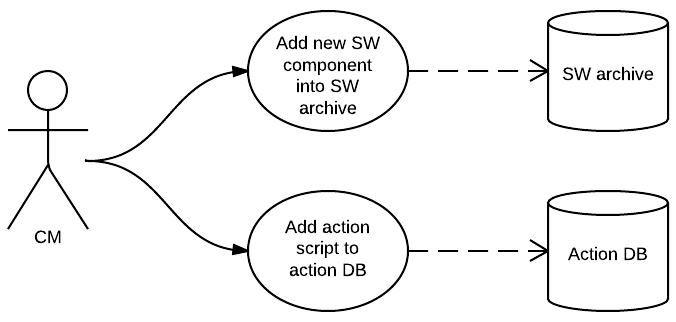
\includegraphics[width=\textwidth]{pics/usecase1.png}
	\end{figure}

	\begin{table}[H]
		\begin{tabular}{ p{4cm} | p{10cm} }
			\hline
			\rowcolor{gray}
			{\bf Use case} & {\bf A new version of a software component} \\ \hline
			{\bf Actors} & CM - Configuration team\\ \hline
			{\bf Application} & Socam \\ \hline
			{\bf Requirements covered} & 1 and 2 \\ \hline
			{\bf Description} & A CM responsible wants to add a new SW-component to the 
			SW archive, the person also have to update the Action DB with the actionscript 
			that connects the SW-component to the ECU.\\ \hline
			{\bf Preconditions} & {\bf 1)} Running computer {\bf 2)} Log on to the system {\bf 3)} ECU already in system\\ \hline
			{\bf Data} & SW + actionscript \\ \hline
			{\bf Stimulus} & A new software component is created by the SW department \\ \hline
			{\bf Flow of events} & 

				\begin{enumerate}[font=\bfseries]
					\item CM enters the new SW component to the system and uploads it to the SW archive
					\begin{enumerate}[label*=\arabic*., font=\bfseries]
						\item CM enters invalid component. 
					\end{enumerate}
					
					\item CM adds the new actionscript and uploads it to the Action DB
					\begin{enumerate}[label*=\arabic*., font=\bfseries]
						\item CM enters invalid actionscript
					\end{enumerate}
				\end{enumerate}
			
			\\ \hline
			{\bf Response} & Both the new SW component and actionscript are 
			successfully uploaded to the respective databases \\ \hline

		\end{tabular}
	\end{table}

\section{Scenario 2}

	\begin{figure}[H]
		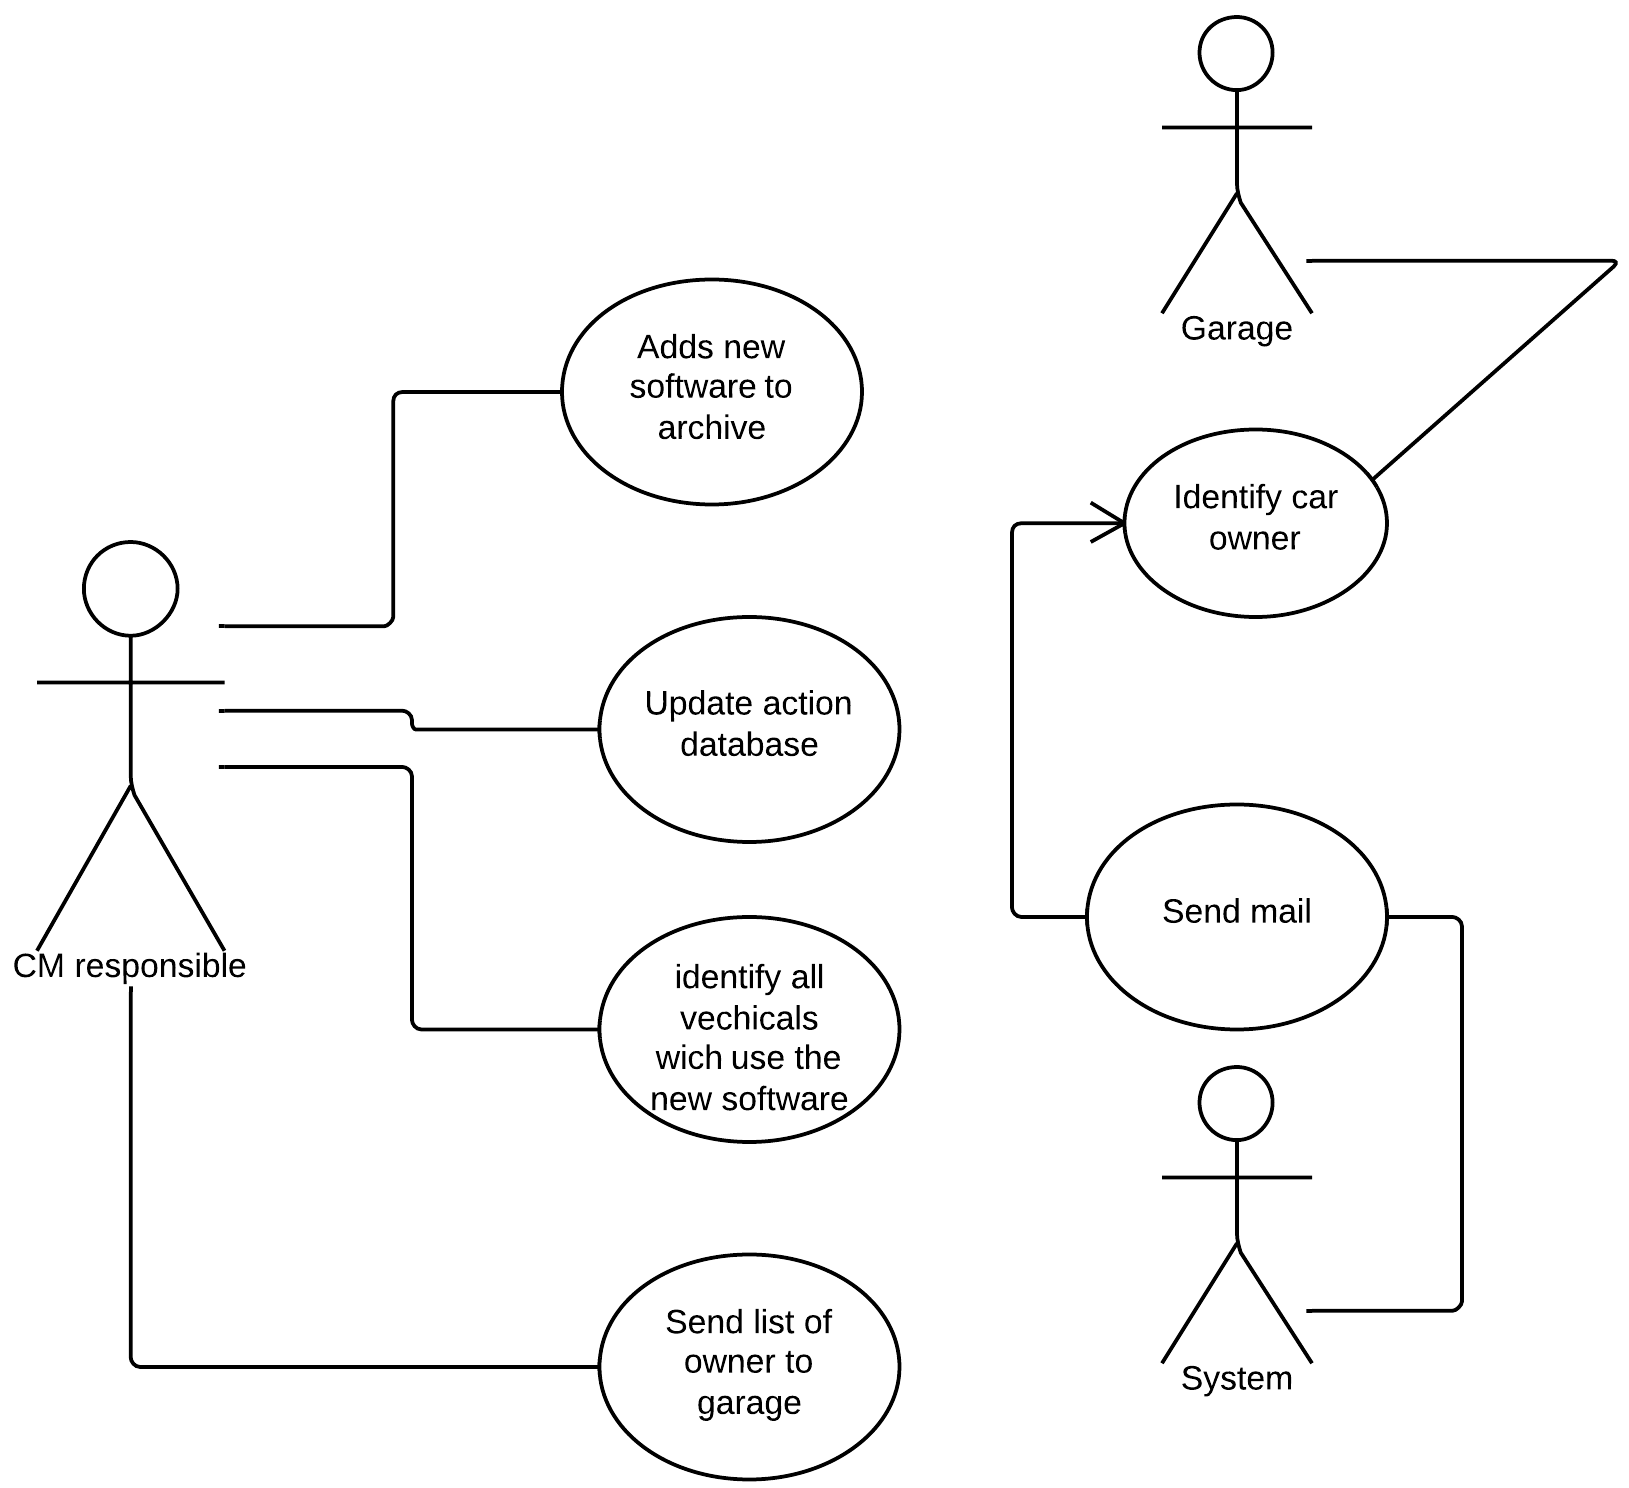
\includegraphics[width=\textwidth]{pics/usecase2.png}
	\end{figure}

	\begin{table}[H]
		\begin{tabular}{ p{4cm} | p{10cm} }
			\hline
			\rowcolor{gray}
			{\bf Use case} & {\bf A safety critical software defect is discovered} \\ \hline
			{\bf Actors} & CM responsible, System, Garage \\ \hline
			{\bf Application} & Socam \\ \hline
			{\bf Requirements covered} & 1, 2, 4 and 5\\ \hline
			{\bf Description} & When a safety critical software defect is discovered a CM 
			responsible will repair the defect and make it availabel in the database. 
			The garage will then make sure that all the relevant carowners get information 
			about the defect and the system improvments.\\ \hline
			{\bf Preconditions} & {\bf 1)} Running computer {\bf 2)} Log on to the system \\ \hline
			{\bf Data} & SW + actionscript \\ \hline
			{\bf Stimulus} & New software is developed \\ \hline
			{\bf Flow of events} & 
				\begin{enumerate}[font=\bfseries]
					\item add new software to the archive
						\begin{enumerate}[label*=\arabic*., font=\bfseries]
							\item The software allready exist 
						\end{enumerate}
					\item update actionscript database
						\begin{enumerate}[label*=\arabic*., font=\bfseries]
							\item Connection to database fails. 
						\end{enumerate}
					\item Identify all vehicles that will be using the new system.
					\item CM responsible logs out
					\item List of vehicles is send to all registered garage.
						\begin{enumerate}[label*=\arabic*., font=\bfseries]
							\item  List of vehicles is not received by the garage.
						\end{enumerate}
					\item Garage employee identifies relevant car owners.
						\begin{enumerate}[label*=\arabic*., font=\bfseries]
							\item Car has no registered owner.
						\end{enumerate}
					\item System makes e-mail that is send to all the car owners.
						\begin{enumerate}[label*=\arabic*., font=\bfseries]
							\item Sending e-mail fails.
						\end{enumerate}
				\end{enumerate}
			
			\\ \hline
			{\bf Response} &  \\ \hline
		\end{tabular}
	\end{table}

\clearpage

\section{Scenario 3}
	
	\begin{figure}[H]
		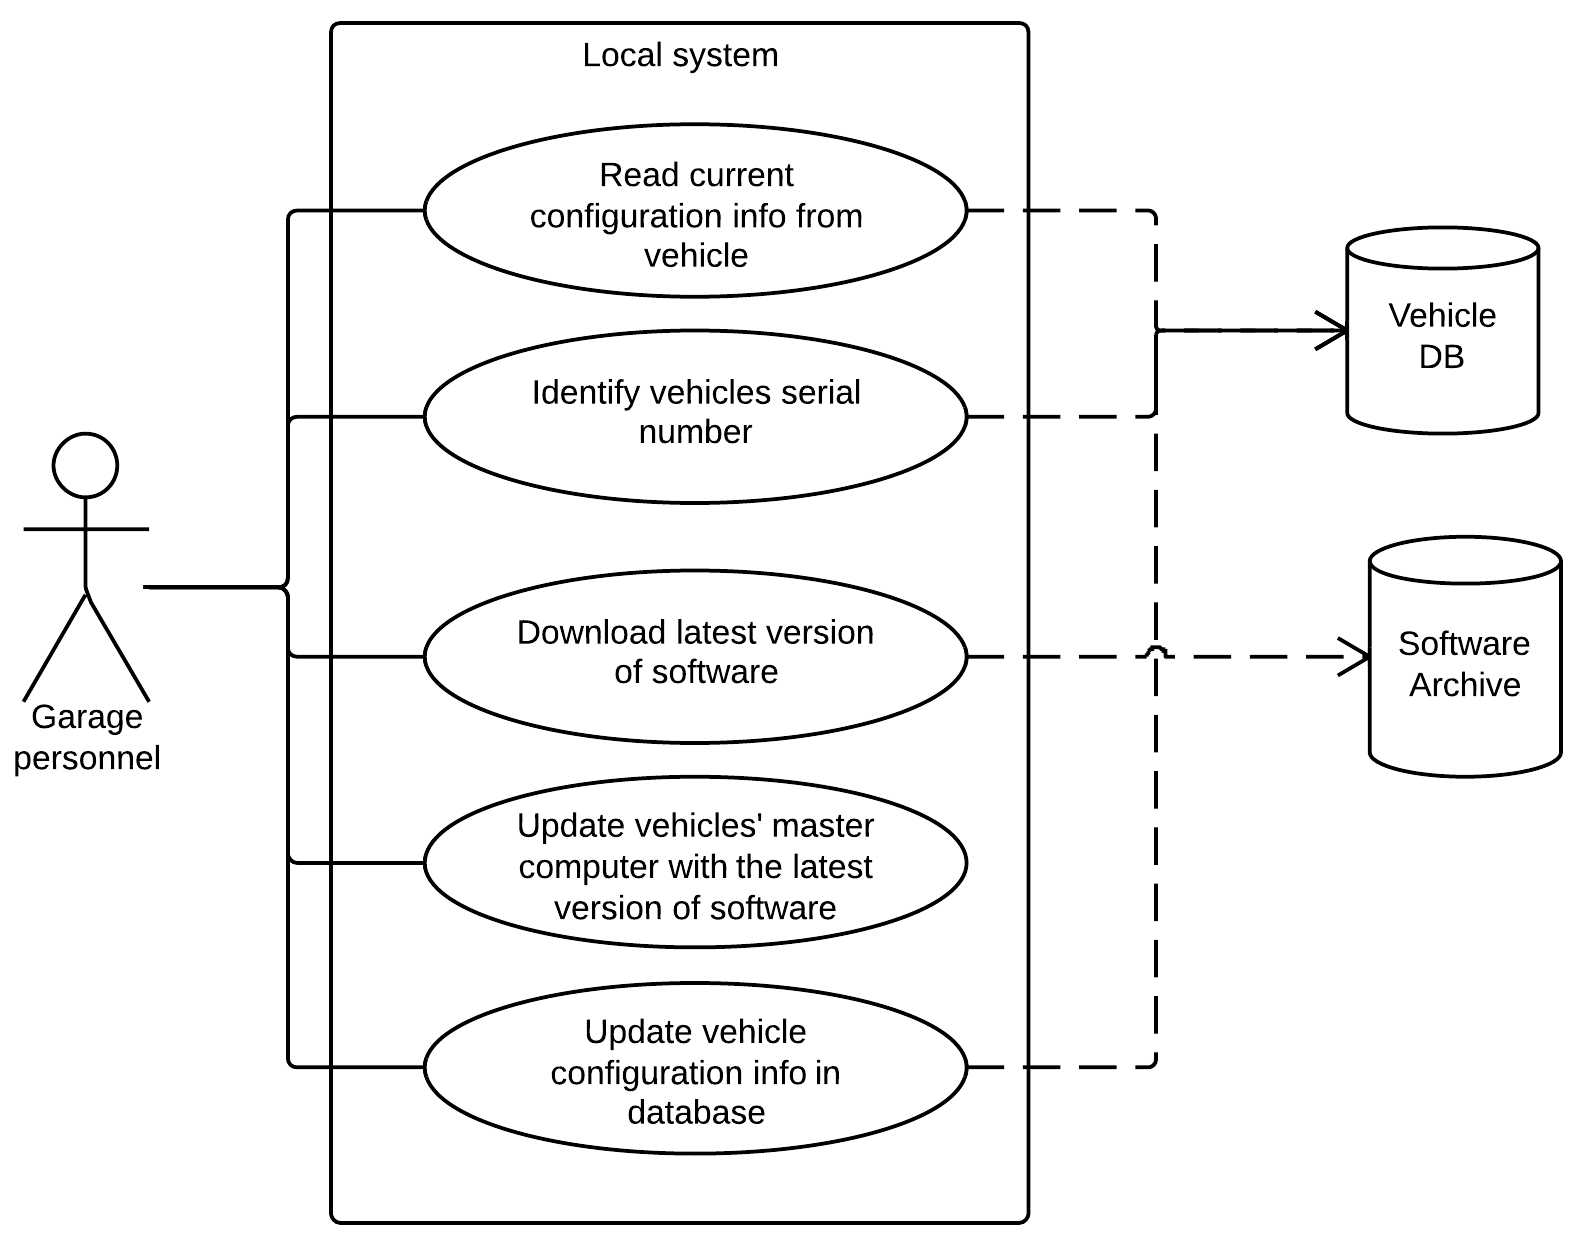
\includegraphics[width=\textwidth]{pics/usecase3.png}
	\end{figure}

		\begin{table}[H]
		\begin{tabular}{ p{4cm} | p{10cm} }
			\hline
			\rowcolor{gray}
			{\bf Use case} & {\bf A vehicle is scheduled for maintanance} \\ \hline
			{\bf Actors} & Garage personnel\\ \hline
			{\bf Application} & Socam \\ \hline
			{\bf Requirements covered} & 6, 7 and 8 \\ \hline
			{\bf Description} & A vehicle is scheduled for maintenance. The vehicle 
			is controlled and updated with the latest version of software. \\ \hline
			{\bf Preconditions} & \\ \hline
			{\bf Data} & Vehicle configuration info, vehicle serial number, software update \\ \hline
			{\bf Stimulus} & A vehicle is scheduled for maintainance \\ \hline
			{\bf Flow of events} & 
				\begin{enumerate}[font=\bfseries]
					\item Read the current configuration info from the vehicle
					\item The garage personnel identifies the vehicles serial 
					number from the owners name.
					\item Downloads the latest version of software 
						\begin{enumerate}[label*=\arabic*., font=\bfseries]
							\item The car is already up to date with the latest software, jump to 6.
						\end{enumerate}
					\item Updates the vehicles master computer with the latest software.
					\item The database is updates with vehicles software updates
					\item Finished
				\end{enumerate}
			
			\\ \hline
			{\bf Response} & Software update successful  \\ \hline

		\end{tabular}
	\end{table}


\clearpage
\section{Scenario 4}

	\begin{figure}[H]
		\centering
		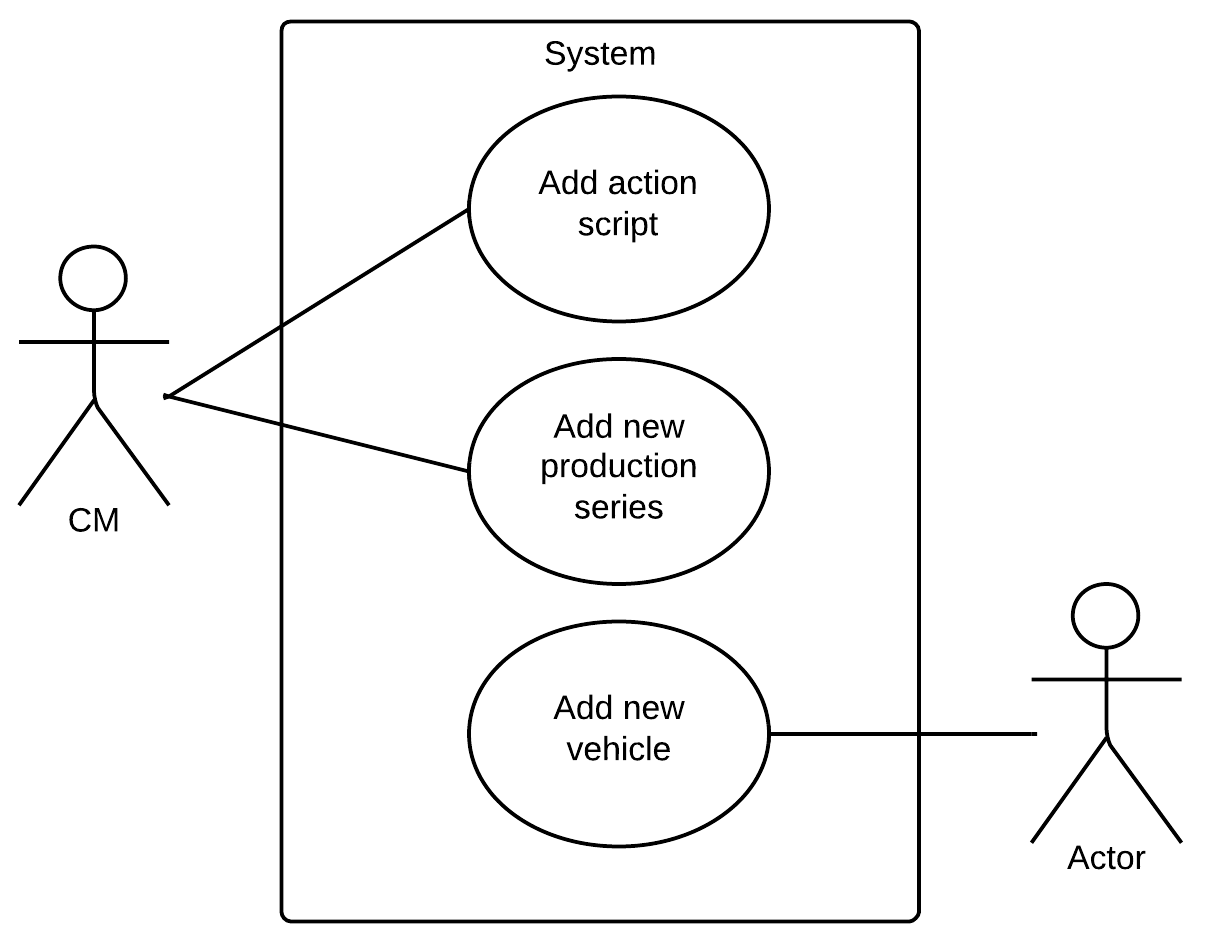
\includegraphics[scale=0.25]{pics/usecase4.png}
	\end{figure}


	\begin{table}[H]
		\centering
		\begin{tabular}{  p{4cm} | p{10cm} }
			\hline
			\rowcolor{gray}
			{\bf Use case} & {\bf A new vehicle is finished from the factory} \\ \hline
			{\bf Actors} & CM - Configuration team, FP - Factory personel \\ \hline
			{\bf Application} & Socam \\ \hline
			{\bf Requirements covered} & 2 and 3 \\ \hline
			{\bf Description} & A new series of vehicle is made and needs to be 
			added into the system \\ \hline
			{\bf Preconditions} & {\bf 1)} Running computer {\bf 2)} Log on to the system \\ \hline
			{\bf Data} & Vehicle series information and specific vehicle \\ \hline
			{\bf Stimulus} & A new vehicle series is added into the system \\ \hline
			{\bf Flow of events} & 
				\begin{enumerate}[font=\bfseries]
					\item CM adds a new action script to the action script database
						\begin{enumerate}[label*=\arabic*., font=\bfseries]
							\item Not valid action script
							\item Not valid parameters given when adding a new vehicle 
							production serie.
							\item Not valid parameters given when adding a new vehicle 
							to the database
							\item Action script is saved with errors
						\end{enumerate}
					\item CM adds the new serie of vehicle to the vehicle database
					\item FP adds a new vehicle to a vehicle production series in the vehicle database. 
				\end{enumerate}
			
			\\ \hline
			{\bf Response} & Confirmation that product has been registered. \\ \hline
		\end{tabular}
	\end{table}